\documentclass[]{elsarticle} %review=doublespace preprint=single 5p=2 column
%%% Begin My package additions %%%%%%%%%%%%%%%%%%%
\usepackage[hyphens]{url}
\usepackage{lineno} % add
\providecommand{\tightlist}{%
  \setlength{\itemsep}{0pt}\setlength{\parskip}{0pt}}

\bibliographystyle{elsarticle-harv}
\biboptions{sort&compress} % For natbib
\usepackage{graphicx}
\usepackage{booktabs} % book-quality tables
%% Redefines the elsarticle footer
%\makeatletter
%\def\ps@pprintTitle{%
% \let\@oddhead\@empty
% \let\@evenhead\@empty
% \def\@oddfoot{\it \hfill\today}%
% \let\@evenfoot\@oddfoot}
%\makeatother

% A modified page layout
\textwidth 6.75in
\oddsidemargin -0.15in
\evensidemargin -0.15in
\textheight 9in
\topmargin -0.5in
%%%%%%%%%%%%%%%% end my additions to header

\usepackage[T1]{fontenc}
\usepackage{lmodern}
\usepackage{amssymb,amsmath}
\usepackage{ifxetex,ifluatex}
\usepackage{fixltx2e} % provides \textsubscript
% use upquote if available, for straight quotes in verbatim environments
\IfFileExists{upquote.sty}{\usepackage{upquote}}{}
\ifnum 0\ifxetex 1\fi\ifluatex 1\fi=0 % if pdftex
  \usepackage[utf8]{inputenc}
\else % if luatex or xelatex
  \usepackage{fontspec}
  \ifxetex
    \usepackage{xltxtra,xunicode}
  \fi
  \defaultfontfeatures{Mapping=tex-text,Scale=MatchLowercase}
  \newcommand{\euro}{€}
\fi
% use microtype if available
\IfFileExists{microtype.sty}{\usepackage{microtype}}{}
\usepackage{color}
\usepackage{fancyvrb}
\newcommand{\VerbBar}{|}
\newcommand{\VERB}{\Verb[commandchars=\\\{\}]}
\DefineVerbatimEnvironment{Highlighting}{Verbatim}{commandchars=\\\{\}}
% Add ',fontsize=\small' for more characters per line
\usepackage{framed}
\definecolor{shadecolor}{RGB}{248,248,248}
\newenvironment{Shaded}{\begin{snugshade}}{\end{snugshade}}
\newcommand{\KeywordTok}[1]{\textcolor[rgb]{0.13,0.29,0.53}{\textbf{{#1}}}}
\newcommand{\DataTypeTok}[1]{\textcolor[rgb]{0.13,0.29,0.53}{{#1}}}
\newcommand{\DecValTok}[1]{\textcolor[rgb]{0.00,0.00,0.81}{{#1}}}
\newcommand{\BaseNTok}[1]{\textcolor[rgb]{0.00,0.00,0.81}{{#1}}}
\newcommand{\FloatTok}[1]{\textcolor[rgb]{0.00,0.00,0.81}{{#1}}}
\newcommand{\ConstantTok}[1]{\textcolor[rgb]{0.00,0.00,0.00}{{#1}}}
\newcommand{\CharTok}[1]{\textcolor[rgb]{0.31,0.60,0.02}{{#1}}}
\newcommand{\SpecialCharTok}[1]{\textcolor[rgb]{0.00,0.00,0.00}{{#1}}}
\newcommand{\StringTok}[1]{\textcolor[rgb]{0.31,0.60,0.02}{{#1}}}
\newcommand{\VerbatimStringTok}[1]{\textcolor[rgb]{0.31,0.60,0.02}{{#1}}}
\newcommand{\SpecialStringTok}[1]{\textcolor[rgb]{0.31,0.60,0.02}{{#1}}}
\newcommand{\ImportTok}[1]{{#1}}
\newcommand{\CommentTok}[1]{\textcolor[rgb]{0.56,0.35,0.01}{\textit{{#1}}}}
\newcommand{\DocumentationTok}[1]{\textcolor[rgb]{0.56,0.35,0.01}{\textbf{\textit{{#1}}}}}
\newcommand{\AnnotationTok}[1]{\textcolor[rgb]{0.56,0.35,0.01}{\textbf{\textit{{#1}}}}}
\newcommand{\CommentVarTok}[1]{\textcolor[rgb]{0.56,0.35,0.01}{\textbf{\textit{{#1}}}}}
\newcommand{\OtherTok}[1]{\textcolor[rgb]{0.56,0.35,0.01}{{#1}}}
\newcommand{\FunctionTok}[1]{\textcolor[rgb]{0.00,0.00,0.00}{{#1}}}
\newcommand{\VariableTok}[1]{\textcolor[rgb]{0.00,0.00,0.00}{{#1}}}
\newcommand{\ControlFlowTok}[1]{\textcolor[rgb]{0.13,0.29,0.53}{\textbf{{#1}}}}
\newcommand{\OperatorTok}[1]{\textcolor[rgb]{0.81,0.36,0.00}{\textbf{{#1}}}}
\newcommand{\BuiltInTok}[1]{{#1}}
\newcommand{\ExtensionTok}[1]{{#1}}
\newcommand{\PreprocessorTok}[1]{\textcolor[rgb]{0.56,0.35,0.01}{\textit{{#1}}}}
\newcommand{\AttributeTok}[1]{\textcolor[rgb]{0.77,0.63,0.00}{{#1}}}
\newcommand{\RegionMarkerTok}[1]{{#1}}
\newcommand{\InformationTok}[1]{\textcolor[rgb]{0.56,0.35,0.01}{\textbf{\textit{{#1}}}}}
\newcommand{\WarningTok}[1]{\textcolor[rgb]{0.56,0.35,0.01}{\textbf{\textit{{#1}}}}}
\newcommand{\AlertTok}[1]{\textcolor[rgb]{0.94,0.16,0.16}{{#1}}}
\newcommand{\ErrorTok}[1]{\textcolor[rgb]{0.64,0.00,0.00}{\textbf{{#1}}}}
\newcommand{\NormalTok}[1]{{#1}}
\usepackage{longtable}
\usepackage{graphicx}
% We will generate all images so they have a width \maxwidth. This means
% that they will get their normal width if they fit onto the page, but
% are scaled down if they would overflow the margins.
\makeatletter
\def\maxwidth{\ifdim\Gin@nat@width>\linewidth\linewidth
\else\Gin@nat@width\fi}
\makeatother
\let\Oldincludegraphics\includegraphics
\renewcommand{\includegraphics}[1]{\Oldincludegraphics[width=\maxwidth]{#1}}
\ifxetex
  \usepackage[setpagesize=false, % page size defined by xetex
              unicode=false, % unicode breaks when used with xetex
              xetex]{hyperref}
\else
  \usepackage[unicode=true]{hyperref}
\fi
\hypersetup{breaklinks=true,
            bookmarks=true,
            pdfauthor={},
            pdftitle={Portfolio Creation \textbar{} Mimicking 10-Year S\&P 500 Returns via DCC Multivariate EGARCH Processes},
            colorlinks=true,
            urlcolor=blue,
            linkcolor=magenta,
            pdfborder={0 0 0}}
\urlstyle{same}  % don't use monospace font for urls
\setlength{\parindent}{0pt}
\setlength{\parskip}{6pt plus 2pt minus 1pt}
\setlength{\emergencystretch}{3em}  % prevent overfull lines
\setcounter{secnumdepth}{0}
% Pandoc toggle for numbering sections (defaults to be off)
\setcounter{secnumdepth}{0}
% Pandoc header


\usepackage[nomarkers]{endfloat}

\begin{document}
\begin{frontmatter}

  \title{Portfolio Creation \textbar{} Mimicking 10-Year S\&P 500 Returns via DCC
Multivariate EGARCH Processes}
    \author[]{Nathan Matare}
  
  
      \address[]{The University of Chicago Booth School of Business}
    \address[Another University]{nmatare@chicagobooth.edu}
  
  \begin{abstract}
  Create a portfolio that best mimics the daily returns of the S\&P 500
  Index over the past 10 years and does not hold more than 10 securities
  at any one time. Securities may consist of individual company stocks and
  not funds nor any other type of investment vehicle.
  \end{abstract}
  
 \end{frontmatter}

\section{Methodology}\label{methodology}

I will mimic the daily returns of the S\&P 500 by isolating and holding
ten securities whose returns are most similar to the S\&P 500 during
each period. This is a non-trivial process, thus I employ Dynamic
Conditional Correlation (DCC) Multivariate Exponential Generalized
Autoregressive Conditional Heteroscedasticity (EGARCH) models to
identify and isolate similar return-yielding securities for each period
throughout the 10-year sample.

The process outline is such:

\begin{enumerate}
\def\labelenumi{\arabic{enumi}.}
\tightlist
\item
  Collect daily price levels on S\&P 500 secruities;
\item
  Clean and pre-process data;
\item
  Estimate time varying conditional correlation via eGARCH and DCC
  models;
\item
  Isolate the top-ten most correlated securities and form a daily
  portfolio; and
\item
  Compare portfolio returns to S\&P 500 returns.
\end{enumerate}

Project Summary:

First, a targeted universe of securities is generated. Next, raw price
levels are cleaned, logged, and first-order integrated. Several GARCH
models are considered \footnote{SGARCH, APARCH, GJR-GARCH, EGARCH} in
order to best capture the variance dynamics in each time series. After
completion, an appropriate VAR DCC model is fit to the security and
market time-series data. Next, the top-ten most correlated securities
are selected and inputed into the final portfolio. Finally, the
portfolio returns are compared against the daily S\&P 500 returns.

\section{Collect Daily Price Levels}\label{collect-daily-price-levels}

I begin by compiling a list of all stocks currently listed on the S\&P
500. These stocks constitute the `universe of securities' and form the
basis of candidate stocks. In order to expedite the collection of
granular price series data, I program the function ``SecurityScraper''
\footnote{See appendix for additional information} to integrate with
Quandl.com's API and scrape daily price level data for the past 10
years.\footnote{See \href{https://www.quandl.com/data/WIKI}{Quandl}
  datasets}

\begin{Shaded}
\begin{Highlighting}[]
\NormalTok{enddate <-}\StringTok{ }\KeywordTok{Sys.Date}\NormalTok{()}
\NormalTok{startdate <-}\StringTok{ }\NormalTok{enddate -}\StringTok{ }\DecValTok{365}\NormalTok{*}\DecValTok{10} 
\KeywordTok{source}\NormalTok{(}\StringTok{"secruityscraper.R"}\NormalTok{)}
\KeywordTok{SecruityScraper}\NormalTok{(}\DataTypeTok{name=}\StringTok{"SP500"}\NormalTok{, }
                \DataTypeTok{startdate=}\NormalTok{startdate, }
                \DataTypeTok{enddate=}\NormalTok{enddate, }\DataTypeTok{type=}\StringTok{"WIKI"}\NormalTok{, }
                \DataTypeTok{key=}\StringTok{"X"}\NormalTok{, }\DataTypeTok{sleep=}\DecValTok{0}\NormalTok{)}
\end{Highlighting}
\end{Shaded}

\section{Collect Daily Price Levels}\label{collect-daily-price-levels-1}

The collected 10MB raw dataset contains weekends, holidays, and missing
observations. It is necessary to clean and pre-process the data in order
to facilitate smooth analysis. I deploy another function,
``SecruityCleaner'' \footnote{See appendix for additional information}
to clean the data. \footnote{Missing observations are imputed with
  either the nearest column value or column mean, dependent on the
  situation, see appendix for code logic} Securities with too few
observations are removed from the candidate pool; the universe of
potential securities totals 474 stocks with 2514 daily observations.

\begin{Shaded}
\begin{Highlighting}[]
\KeywordTok{source}\NormalTok{(}\StringTok{"secruitycleaner.R"}\NormalTok{)}
\KeywordTok{SecruityCleaner}\NormalTok{(}\DataTypeTok{name=}\StringTok{"SP500"}\NormalTok{, }\DataTypeTok{days=}\DecValTok{144}\NormalTok{)}
\end{Highlighting}
\end{Shaded}

Additionally, I append daily S\&P 500 price levels to the dataset:

\begin{Shaded}
\begin{Highlighting}[]
\NormalTok{sp <-}\StringTok{ }\KeywordTok{Quandl}\NormalTok{(}\StringTok{"YAHOO/INDEX_GSPC"}\NormalTok{, }\DataTypeTok{start_date=}\NormalTok{startdate, }\DataTypeTok{end_date=}\NormalTok{enddate)}
\NormalTok{rows <-}\StringTok{ }\KeywordTok{match}\NormalTok{(}\KeywordTok{as.character}\NormalTok{(sp[,}\DecValTok{1}\NormalTok{]), }\KeywordTok{as.character}\NormalTok{(raw[,}\DecValTok{1}\NormalTok{])) }\CommentTok{#match SP levels to clean dataset}
\NormalTok{raw$SP500 <-}\StringTok{ }\NormalTok{sp[,}\DecValTok{2}\NormalTok{] }\CommentTok{#append S&P 500 to vector }
\end{Highlighting}
\end{Shaded}

Now that the dataset contains the entire universe of cleaned price
levels, I further transform the data via a natural log and first-order
integration. Such transformation grants an advantageous property of
approximating continuously compounding returns:
\[r=ln(p_{t}) - ln(p_{t-1})\]

\begin{Shaded}
\begin{Highlighting}[]
\CommentTok{#Convert data to log level and take difference}
\NormalTok{data <-}\StringTok{ }\KeywordTok{data.frame}\NormalTok{(}\KeywordTok{apply}\NormalTok{(raw[,-}\DecValTok{1}\NormalTok{], }\DataTypeTok{MARGIN=}\DecValTok{2}\NormalTok{, log)) }
\NormalTok{data$Date <-}\StringTok{ }\KeywordTok{as.character}\NormalTok{(dates)}

\CommentTok{#Difference log prices to find returns }
\NormalTok{rtrn <-}\StringTok{ }\KeywordTok{data.frame}\NormalTok{(}\KeywordTok{apply}\NormalTok{(data[,-}\KeywordTok{dim}\NormalTok{(data)[}\DecValTok{2}\NormalTok{]], }\DataTypeTok{MARGIN=}\DecValTok{2}\NormalTok{, diff)) }
\NormalTok{rtrn$Date <-}\StringTok{ }\KeywordTok{as.character}\NormalTok{(dates[-}\DecValTok{1}\NormalTok{])}
\KeywordTok{rownames}\NormalTok{(rtrn) <-}\StringTok{ }\NormalTok{sp$Date[-}\DecValTok{1}\NormalTok{]}
\end{Highlighting}
\end{Shaded}

\section{Analysis: Univariate Variance
Modeling}\label{analysis-univariate-variance-modeling}

The following analysis will become computationally expensive, I
instantiate a parallel environment to increase the speed of computation.

\begin{Shaded}
\begin{Highlighting}[]
\KeywordTok{library}\NormalTok{(parallel)}
\NormalTok{cl <-}\StringTok{ }\KeywordTok{makeCluster}\NormalTok{(}\KeywordTok{min}\NormalTok{(}\KeywordTok{detectCores}\NormalTok{(),}\DecValTok{5}\NormalTok{), }\DataTypeTok{type=}\KeywordTok{ifelse}\NormalTok{(.Platform$OS.type==}\StringTok{"unix"}\NormalTok{,}\StringTok{"FORK"}\NormalTok{,}\StringTok{"PSOCK"}\NormalTok{))}
\end{Highlighting}
\end{Shaded}

Before fitting GARCH models, I inspect several return series. For the
S\&P 500 series, I observe non-normality, heavy kurtosis, and slight
negative skew. Given that standard GARCH models assume
\textasciitilde{}N(0,1) errors, I caution against the standard
model---it may be necessary to adjust the distribution parameters to
account for the skewed non-normality. Similar analysis and conclusions
follow for individual stock variance distributions.

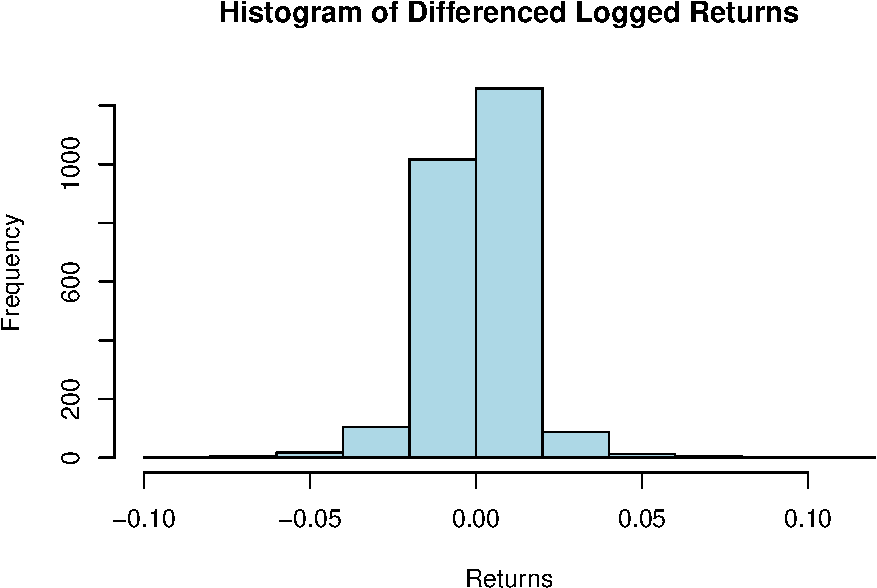
\includegraphics{report_files/figure-latex/analysis11-1.pdf}

\begin{Shaded}
\begin{Highlighting}[]
\KeywordTok{kurtosis}\NormalTok{(moddata[,}\DecValTok{1}\NormalTok{])}
\end{Highlighting}
\end{Shaded}

\begin{verbatim}
## [1] 12.93363
\end{verbatim}

\begin{Shaded}
\begin{Highlighting}[]
\KeywordTok{skewness}\NormalTok{(moddata[,}\DecValTok{1}\NormalTok{])}
\end{Highlighting}
\end{Shaded}

\begin{verbatim}
## [1] -0.3189841
\end{verbatim}

Thus, to account for non-normality and left skew, I vary model
parameters in an attempt to capture the underlying dynamics. I begin by
adjusting distribution parameters: normal, normal-skewed,
t-distribution, t-skewed; before settling on a normal distribution. It
appears that while the data may not be perfectly normal---the normal
distribution, in-fact, captures the underlying process more sufficiently
than any other available distribution.

Further, standard GARCH models assume symmetry between negative and
positive returns. That is, previous period positive returns affect
current period variance at the same magnitude as previous period
negative returns. However, empirical research suggests otherwise;
indeed, previous period negative returns affect current period variance
at a greater magnitude than previous period positive returns. Thus, I
introduce several asymmetric models, namely: EGARCH, GJR-GARCH,
APARCH\footnote{http://public.econ.duke.edu/\textasciitilde{}boller/Papers/glossary\_arch.pdf},
before determining through model diagnostics that an exponential GARCH
is the best candidate.\footnote{While an GJR-GARCH process fit the
  series better---matrix singularities when the model is piped into the
  VAR DCC model force me to select an EGARCH process}

\[\log\sigma_{t}^2=\omega+\sum_{k=1}^{q}\beta_{k}g(Z_{t-k})+\sum_{k=1}^{p}\alpha_{k}\log\sigma_{t-k}^{2}\]

Although I am able to manually determine that an EGARCH(2,2) process
passes all diagnostic tests and fits the S\&P 500 series sufficiently,
it is time prohibitive to replicate this manual process for all
individual secruities. I could automate this process and select the most
advantageous EGARCH(p,q) model based upon residual, autocorrelation
function (ACF), partial autocorrelation function (PACF), and information
criteria; but given time constraints, I settle on an EGARCH(1,1) process
for all individual securities.

\begin{Shaded}
\begin{Highlighting}[]
\KeywordTok{library}\NormalTok{(rmgarch)}
\KeywordTok{require}\NormalTok{(rugarch)}

\CommentTok{#Build parameters for market GARCH}
        \NormalTok{spec1 <-}\StringTok{ }\KeywordTok{ugarchspec}\NormalTok{(}\DataTypeTok{variance.model =} \KeywordTok{list}\NormalTok{(}\DataTypeTok{model =} \StringTok{"eGARCH"}\NormalTok{, }\DataTypeTok{garchOrder =} \KeywordTok{c}\NormalTok{(}\DecValTok{2}\NormalTok{,}\DecValTok{2}\NormalTok{)),}
                                \DataTypeTok{distribution.model=} \StringTok{"norm"}\NormalTok{)}
\CommentTok{#Build parameters for secruity GARCH}
        \NormalTok{spec2 <-}\StringTok{ }\KeywordTok{ugarchspec}\NormalTok{(}\DataTypeTok{variance.model =} \KeywordTok{list}\NormalTok{(}\DataTypeTok{model =} \StringTok{"eGARCH"}\NormalTok{, }\DataTypeTok{garchOrder =} \KeywordTok{c}\NormalTok{(}\DecValTok{1}\NormalTok{,}\DecValTok{1}\NormalTok{)),}
                                \DataTypeTok{distribution.model=} \StringTok{"norm"}\NormalTok{)}
\CommentTok{#Fit GARCH models}
        \NormalTok{garch1 <-}\StringTok{ }\KeywordTok{ugarchfit}\NormalTok{(}\DataTypeTok{spec=}\NormalTok{spec1, }\DataTypeTok{data=}\NormalTok{moddata[,}\DecValTok{1}\NormalTok{], }\DataTypeTok{solver.control =} \KeywordTok{list}\NormalTok{(}\DataTypeTok{trace=}\DecValTok{0}\NormalTok{), }
                            \DataTypeTok{cluster=}\NormalTok{cl)}
        \NormalTok{garch2 <-}\StringTok{ }\KeywordTok{try}\NormalTok{(}\KeywordTok{ugarchfit}\NormalTok{(}\DataTypeTok{spec=}\NormalTok{spec2, }\DataTypeTok{data=}\NormalTok{moddata[,}\DecValTok{2}\NormalTok{], }\DataTypeTok{solver.control =} \KeywordTok{list}\NormalTok{(}\DataTypeTok{trace=}\DecValTok{0}\NormalTok{), }
                            \DataTypeTok{cluster=}\NormalTok{cl), }\DataTypeTok{silent=}\OtherTok{TRUE}\NormalTok{)}
\end{Highlighting}
\end{Shaded}

Graphic displays of diagnostic checks and assumptions follow:\footnote{The
  dates in the below plots are incorrect; the rmgarch package has an
  error that defaults to this time period}

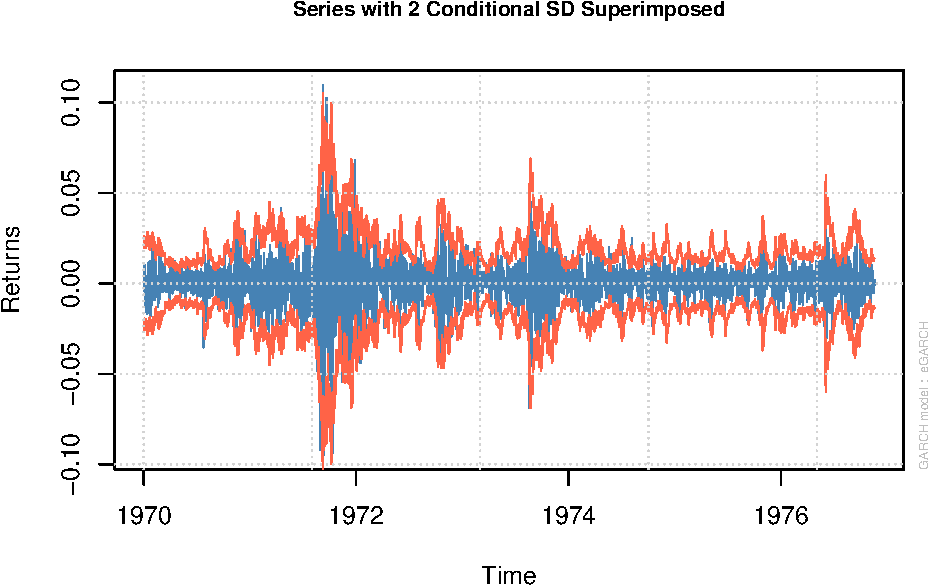
\includegraphics{report_files/figure-latex/analysis201-1.pdf}

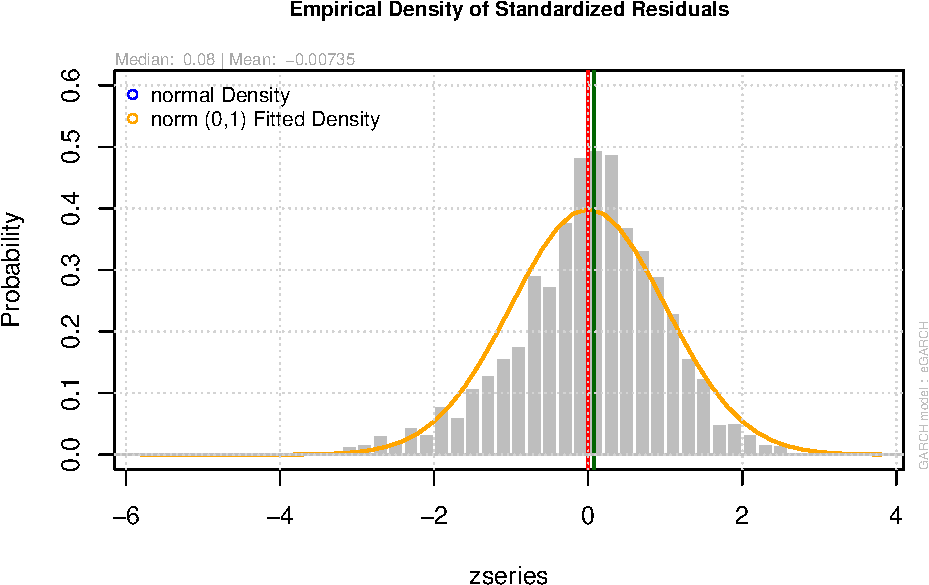
\includegraphics{report_files/figure-latex/analysis20df1-1.pdf}

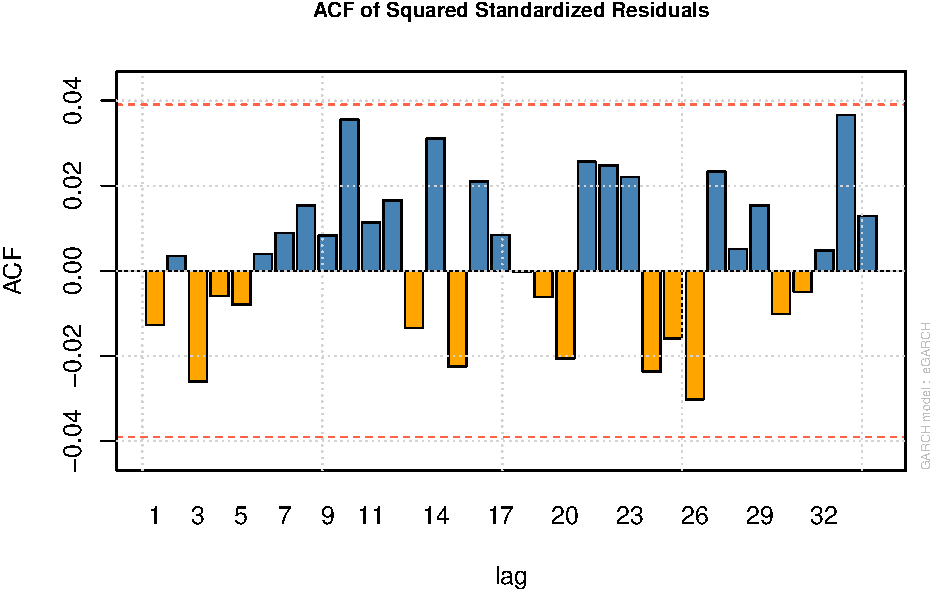
\includegraphics{report_files/figure-latex/analysis2031-1.pdf}

As discussed previously, residual diagnostics reveal that the errors are
not \textasciitilde{}N(0,1) I.D. Adjusting otherwise worsen the errors.

\begin{Shaded}
\begin{Highlighting}[]
\KeywordTok{kurtosis}\NormalTok{(garch1@fit$residuals)}
\end{Highlighting}
\end{Shaded}

\begin{verbatim}
## [1] 12.63651
\end{verbatim}

\begin{Shaded}
\begin{Highlighting}[]
\KeywordTok{skewness}\NormalTok{(garch1@fit$residuals)}
\end{Highlighting}
\end{Shaded}

\begin{verbatim}
## [1] -0.4385969
\end{verbatim}

\begin{longtable}[c]{@{}lrrrr@{}}
\toprule
& Estimate & Std. Error & t value &
Pr(\textgreater{}\textbar{}t\textbar{})\tabularnewline
\midrule
\endhead
mu & 0.0002682 & 0.0001182 & 2.269900 & 0.0232137\tabularnewline
ar1 & 0.3271671 & 0.0554327 & 5.902059 & 0.0000000\tabularnewline
ma1 & -0.3909436 & 0.0537169 & -7.277854 & 0.0000000\tabularnewline
omega & -0.2859863 & 0.0179554 & -15.927569 & 0.0000000\tabularnewline
alpha1 & -0.2968012 & 0.0303461 & -9.780529 & 0.0000000\tabularnewline
alpha2 & 0.1269753 & 0.0272309 & 4.662917 & 0.0000031\tabularnewline
beta1 & 0.9999999 & 0.0000088 & 113420.181733 & 0.0000000\tabularnewline
beta2 & -0.0312999 & 0.0019570 & -15.993674 & 0.0000000\tabularnewline
gamma1 & -0.1449825 & 0.0391676 & -3.701592 & 0.0002143\tabularnewline
gamma2 & 0.2973042 & 0.0425145 & 6.993006 & 0.0000000\tabularnewline
\bottomrule
\end{longtable}

Upon inspection of the EGARCH(2,2) S\&P 500 process, I observe highly
significant covariates. Notably, the asymmetric terms(gamma(1),
gamma(2)) are highly significant. It appears that the variance may be
non-stationary. The beta(1) coefficient is nearly 1 with an extremely
high t-stat---indicative of a random walk process. Intuitively this
appears spurious---variance, one would expect, should not arbitrary
depart and wander from a mean-level. All other coefficients appear
proper.

\begin{longtable}[c]{@{}lrrrr@{}}
\toprule
& Estimate & Std. Error & t value &
Pr(\textgreater{}\textbar{}t\textbar{})\tabularnewline
\midrule
\endhead
mu & 0.0000000 & 0.0000006 & 0.0000047 & 0.9999962\tabularnewline
ar1 & 0.3685570 & 0.0319029 & 11.5524440 & 0.0000000\tabularnewline
ma1 & -0.6756093 & 0.0083962 & -80.4663500 & 0.0000000\tabularnewline
omega & -0.4826973 & 0.0193245 & -24.9785618 & 0.0000000\tabularnewline
alpha1 & 0.1133147 & 0.0264116 & 4.2903325 & 0.0000178\tabularnewline
beta1 & 0.9002138 & 0.0012210 & 737.2798943 & 0.0000000\tabularnewline
gamma1 & 1.4878254 & 0.0442731 & 33.6056502 & 0.0000000\tabularnewline
\bottomrule
\end{longtable}

Upon inspection of the EGARCH(1,1) individual security process, I
observe mostly significant covariates. Again, the asymmetric term
gamma(1) is highly significant. While the spurious beta coefficient is
no longer observed, the mean-level error term (mu) is highly
insignificant. Indicative of the aforementioned non-normal issues.
Unlike the static S\&P 500 EGARCH(2,2) model, this EGARCH(1,1) model is
fit to all individual securities and may not be the most appropriate
process. However, given resource constraints I continue otherwise.
\footnote{After continually running the entire analysis, a EGARCH(2,2)
  S\&P 500 process in-conjunction with a GJR-GARCH(1,1) individual
  security process produces the lowest error rate; I remain with the
  EGARCH process however, given the robust diagnostic checks}

\section{Analysis: Multivariate Dynamic Conditional
Correlations}\label{analysis-multivariate-dynamic-conditional-correlations}

With the estimated univariate EGARCH(2,2) and EGARCH(1,1) models, I am
ready to incorporate the asymmetric conditional variance into a
multivariate dynamically conditioned vector auto-regression (VAR).
Intuitively, when the S\&P 500 index and individual security move in the
same direction, as measured by variance and returns, the correlation
increases slightly. The opposite holds if both the index and security
move in opposite directions. As with variance estimations, correlations
are assumed to only temporarily deviate from a long run mean---as
indicated by the omega parameter. Further, given asymmetry in the
correlation dynamics, these increased(decreased) correlations should be
exacerbated in economic up(down) turns.

Thus, I consider both a DCC and an ADCC (asymmetric) VAR:

\[\rho_{t} = \bar\rho(1-\alpha-\beta)+\alpha z_{1,t-1}z_{2,t-1} + \beta\rho_{t-1}\]

\[\rho_{t} = \omega + \alpha z_{1,t-1}z_{2,t-1} + \gamma z_{1,t-1}z_{2,t-1}+(I_{z_{1t}<0})(I_{z_{2t}<0})+\beta\rho_{t-1}\]

Diagnostic checks indicate that the asymmetric correlation term is
insignificant for most pairs; I discard the ADCC model. Through AIC/BIC
selection criteria, I determine that a DCC(1,1) model is most
appropriate for the data.\footnote{While higher order DCC models have
  comparable AIC/BIC scores and decreased residual errors, the higher
  order lagged coefficients are deemed insignificant. With caution
  towards over-fitting, I hold a DCC(1,1) process.}

After fitting the model, I aggregate the correlation list into a matrix
and terminate the parallel cluster.

\begin{Shaded}
\begin{Highlighting}[]
\CommentTok{#Build parameters for DCC model }
\NormalTok{dccspec <-}\StringTok{ }\KeywordTok{dccspec}\NormalTok{(}\DataTypeTok{VAR=}\OtherTok{TRUE}\NormalTok{, }\DataTypeTok{uspec =} \KeywordTok{multispec}\NormalTok{(}\KeywordTok{c}\NormalTok{(spec1, spec2)), }\DataTypeTok{dccOrder =} \KeywordTok{c}\NormalTok{(}\DecValTok{1}\NormalTok{,}\DecValTok{1}\NormalTok{), }
                   \DataTypeTok{distribution =} \StringTok{"mvnorm"}\NormalTok{)}

\CommentTok{#Fit DCC model}
\NormalTok{dcc <-}\StringTok{ }\KeywordTok{try}\NormalTok{(}\KeywordTok{dccfit}\NormalTok{(dccspec, }\DataTypeTok{data =} \NormalTok{moddata, }\DataTypeTok{fit.control=}\KeywordTok{list}\NormalTok{(}\DataTypeTok{scale=}\OtherTok{TRUE}\NormalTok{), }\DataTypeTok{cluster=}\NormalTok{cl), }
           \DataTypeTok{silent=}\OtherTok{TRUE}\NormalTok{)}

\NormalTok{corrmatrix <-}\StringTok{ }\KeywordTok{rcor}\NormalTok{(dcc, }\DataTypeTok{type=}\StringTok{"R"}\NormalTok{)}
\NormalTok{corrmatrix <-}\StringTok{ }\KeywordTok{zoo}\NormalTok{(corrmatrix[}\DecValTok{1}\NormalTok{,}\DecValTok{2}\NormalTok{,], }\DataTypeTok{order.by=}\KeywordTok{as.Date}\NormalTok{(}\KeywordTok{rownames}\NormalTok{(moddata)))}
\NormalTok{timevarcor[,n] <-}\StringTok{ }\NormalTok{corrmatrix}

\KeywordTok{stopCluster}\NormalTok{(cl) }
\end{Highlighting}
\end{Shaded}

\begin{center}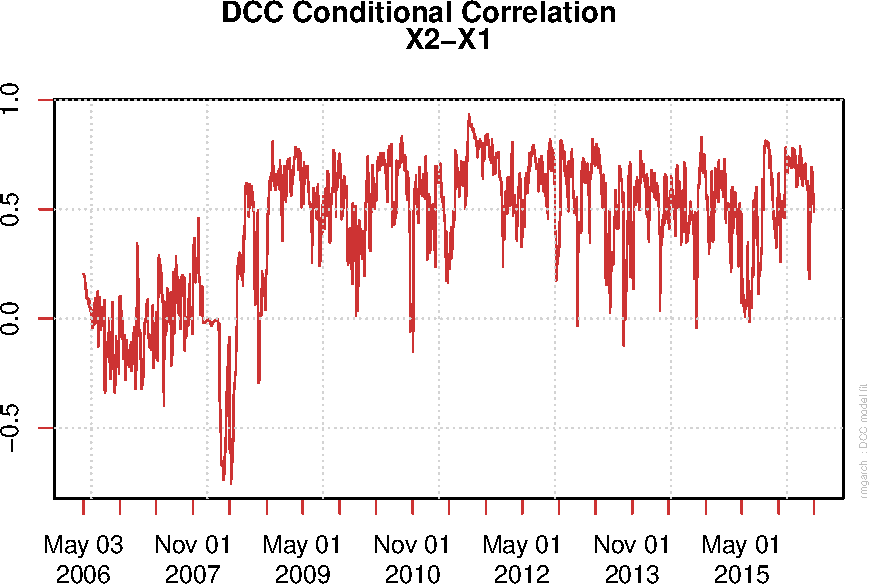
\includegraphics{report_files/figure-latex/analysis232011-1} \end{center}

Upon inspection, the multivariate DCC(1,1) VAR formed from a EGARCH(1,1)
and EGARCH(2,2) process yields mostly significant coefficients. As
previously discussed, several coefficients appear insignificant.
Otherwise, the model appears to capture the dynamically conditioned
correlation well.

\begin{longtable}[c]{@{}lrrrr@{}}
\toprule
& Estimate & Std. Error & t value &
Pr(\textgreater{}\textbar{}t\textbar{})\tabularnewline
\midrule
\endhead
{[}X1{]}.omega & -0.2812474 & 0.0478390 & -5.8790349 &
0.0000000\tabularnewline
{[}X1{]}.alpha1 & -0.2931646 & 0.0282848 & -10.3647370 &
0.0000000\tabularnewline
{[}X1{]}.alpha2 & 0.1245218 & 0.0278806 & 4.4662556 &
0.0000080\tabularnewline
{[}X1{]}.beta1 & 1.0000000 & 0.0000232 & 43143.5149533 &
0.0000000\tabularnewline
{[}X1{]}.beta2 & -0.0309803 & 0.0052412 & -5.9109612 &
0.0000000\tabularnewline
{[}X1{]}.gamma1 & -0.1388295 & 0.0202280 & -6.8632455 &
0.0000000\tabularnewline
{[}X1{]}.gamma2 & 0.2874979 & 0.0294032 & 9.7777600 &
0.0000000\tabularnewline
{[}X2{]}.omega & -0.0115805 & 0.0208363 & -0.5557843 &
0.5783584\tabularnewline
{[}X2{]}.alpha1 & -0.0448929 & 0.1792462 & -0.2504539 &
0.8022364\tabularnewline
{[}X2{]}.beta1 & 0.9977422 & 0.0016093 & 620.0005213 &
0.0000000\tabularnewline
{[}X2{]}.gamma1 & 0.1383119 & 0.1087630 & 1.2716814 &
0.2034863\tabularnewline
{[}Joint{]}dcca1 & 0.1147132 & 0.0295329 & 3.8842557 &
0.0001026\tabularnewline
{[}Joint{]}dccb1 & 0.8813116 & 0.0311983 & 28.2486921 &
0.0000000\tabularnewline
\bottomrule
\end{longtable}

\section{Analysis: Portfolio Evaluation
I}\label{analysis-portfolio-evaluation-i}

From the 20MB csv file containing the dynamically conditioned time
varying correlation for all 474 securities, I select the ten-most
correlated securities (to the S\&P 500) for each period. Put another
way, for each period in the sample, I select the ten-most correlated
securities; the ten-most correlated securities then form the mimicking
portfolio. I lookup the returns for each security per period and equally
weight each individual security's return against the entire portfolio.
This is a rather naive approach; I am essentially equally weighting each
security under the assumption that the overall portfolio will mirror the
S\&P 500's returns well. A more pragmatic approach would be to optimally
weight each individual security's return based upon some intrinsic
property---say regime or security characteristic.

\begin{Shaded}
\begin{Highlighting}[]
\NormalTok{top10names <-}\StringTok{ }\KeywordTok{apply}\NormalTok{(timevarcor[,-}\DecValTok{1}\NormalTok{], }\DataTypeTok{MARGIN=}\DecValTok{1}\NormalTok{, }\DataTypeTok{FUN=}\NormalTok{function(x) }
                   \KeywordTok{names}\NormalTok{(}\KeywordTok{head}\NormalTok{(}\KeywordTok{sort}\NormalTok{(x, }\DataTypeTok{decreasing =} \DataTypeTok{decreasing=}\OtherTok{TRUE}\NormalTok{),}\DecValTok{10}\NormalTok{)))}

\CommentTok{#Compare returns against SP&500 Returns}
\NormalTok{L <-}\StringTok{ }\KeywordTok{dim}\NormalTok{(top10names)[}\DecValTok{2}\NormalTok{]}
\NormalTok{eval <-}\StringTok{ }\KeywordTok{data.frame}\NormalTok{(}\DataTypeTok{Date=}\NormalTok{sp$Date[-}\DecValTok{1}\NormalTok{])}
\NormalTok{eval$SP500 <-}\StringTok{ }\NormalTok{rtrn[,}\DecValTok{474}\NormalTok{]}
\NormalTok{eval$benchmark <-}\StringTok{ }\OtherTok{NA}

\NormalTok{for(n in }\DecValTok{1}\NormalTok{:L)\{}
    \NormalTok{date <-}\StringTok{ }\KeywordTok{names}\NormalTok{(top10names[}\DecValTok{1}\NormalTok{,n])}
    \NormalTok{topstocks <-}\StringTok{ }\KeywordTok{as.character}\NormalTok{(top10names[,n])}
    \NormalTok{lowstocks <-}\StringTok{ }\KeywordTok{as.character}\NormalTok{(low10names[,n])}

    \NormalTok{eval$benchmark[n] <-}\StringTok{ }\KeywordTok{mean}\NormalTok{(}\KeywordTok{as.numeric}\NormalTok{(rtrn[date,topstocks]))}
\NormalTok{\}}
\NormalTok{eval$error <-}\StringTok{ }\NormalTok{eval$SP500 -}\StringTok{ }\NormalTok{eval$benchmark }
\end{Highlighting}
\end{Shaded}

I now have a vector of portfolio returns for each period in the 10-year
sample. I directly compare the performance and error\footnote{The
  eval\$error vector stores the difference between the returns from the
  portfolio and the S\&P 500, IE the `residual' error} of this portfolio
to the S\&P 500 index.

\section{Analysis: Portfolio Evaluation
II}\label{analysis-portfolio-evaluation-ii}

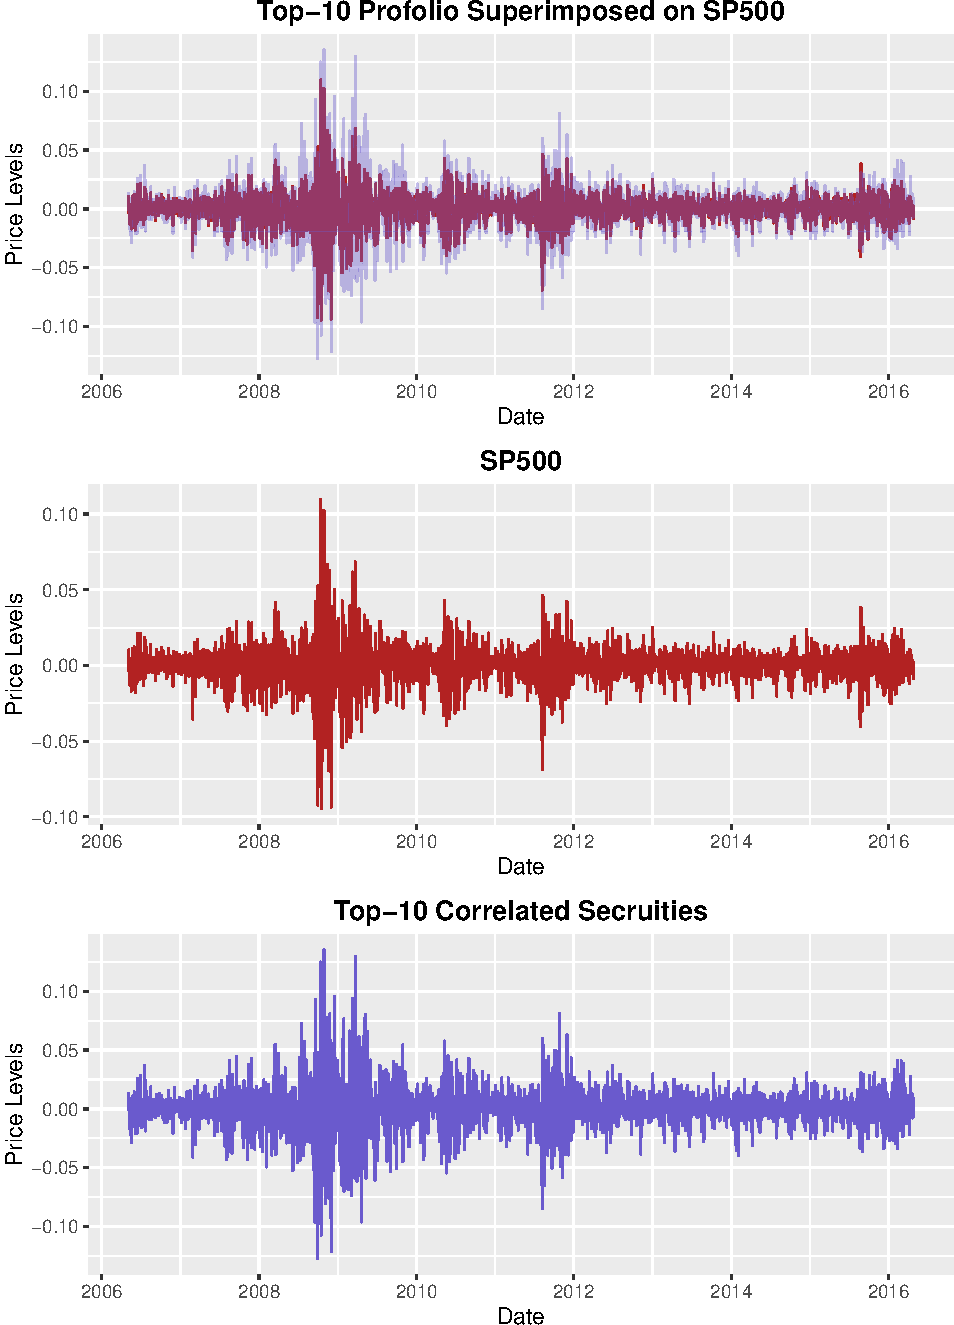
\includegraphics{report_files/figure-latex/analysis23223d011-1.pdf}

The constructed portfolio adequately mimics the returns of the S\&P 500;
the bottommost graph displays the constructed returns. The middle graph
displays the S\&P 500 returns. And the topmost graph displays the
portfolio returns superimposed against the S\&P 500 returns. The EGARCH
DCC VAR selected portfolio adequately mirrors the S\&P 500 benchmark;
however, during regimes of high volatility the residual errors are far
greater than during periods of relatively tranquility. This is rather
intuitive, correlation and variance are tough to estimate during highly
unpredictably periods.

I now quantify the accuracy of the tracking portfolio via a Sharpe
Ratio:

\[S_a = \frac{E[R_a-R_b]}{\sqrt{\mathrm{var}[R_a-R_b]}} * \sqrt{N}\]

Where N = 221 (number of trading days), Ra = average return, and Rb =
risk free rate

The daily annualized Sharpe Ratio of the S\&P 500 Index over a 10-year
sample is 0.2052 while the daily annualized Sharpe Ratio of the tracking
portfolio is 0.2017. Given that the objective is to mimic the daily
returns of the S\&P 500 (without considering volatility), it is
unsurprising that the tracking portfolio performed worse. The benefits
of diversification are lesser in a ten security portfolio.

I now consider the performance of the tracking portfolio as compared to
the S\&P 500, namely:

\[0.05958 = \frac{E[0.0002585-0.0001821]}{\sqrt{\mathrm{var}[0.0002585-0.0001821]}} * \sqrt{221}\]

Where, Ra= average return of formed portfolio, and Rb = average return
of S\&P 500 benchmark

The tracking portfolio, after considering returns and volatility,
inadvertently outperforms the S\&P 500 index. Finally, I construct a
loosely defined Sum of Square Residuals (SSR) metric. While this metric
is not valuable in isolation---one must re-run the entire analysis and
vary model parameters to achieve insight ---one can use it to compare
across models. Given a multivariate DCC(1,1) \textasciitilde{}N(0,1)
with univariate EGARCH(2,2) \textasciitilde{}N(0,1) and EGARCH(1,1)
\textasciitilde{}N(0,1) process I achieve an `SSR' of 0.1836. \footnote{Given
  multivariate DCC(1,1) \textasciitilde{}N(0,1) with either univariate
  GJR-GARCH(2,2) \textasciitilde{}STD(0,1) and GJR-GARCH(1,1)
  \textasciitilde{}STD(0,1) or GARCH(2,2) \textasciitilde{}N(0,1) and
  GARCH(1,1) \textasciitilde{}N(0,1) this `SSR' reveals 0.1654 and
  0.2043, respectively.}

\begin{Shaded}
\begin{Highlighting}[]
\KeywordTok{sum}\NormalTok{(((eval$error) **}\StringTok{ }\DecValTok{2}\NormalTok{), }\DataTypeTok{na.rm=}\OtherTok{TRUE}\NormalTok{)}
\end{Highlighting}
\end{Shaded}

\begin{verbatim}
## [1] 0.1835966
\end{verbatim}

\section{Appendix}\label{appendix}

\begin{Shaded}
\begin{Highlighting}[]
\NormalTok{SecruityScraper <-}\StringTok{ }\NormalTok{function(name, startdate, enddate, type, key, sleep)\{}

\CommentTok{# Description}
\CommentTok{# This script scraps Quandl.com for data given a date range and symbol list}

\CommentTok{# Arguments}

\CommentTok{#'name' is the name of a csv file containing stock symbols to download #do not include .csv}
\CommentTok{#'startdate' is the start date of data}
\CommentTok{#'enddate' is the end data of data}
\CommentTok{#'type' is the Quandl database header; this should be input as a character  IE 'WIKI'}
\CommentTok{#'key' is the Quandl key}
\CommentTok{#'sleep' is the number of seconds to wait before querying Quandl server}

\CommentTok{# Example}
\CommentTok{# SecruityScraper("NASDAQ", "2001-09-11", "2015-01-01", "WIKI","40F..U&E")}

\CommentTok{# Requirements}

\CommentTok{# Requires the Quandl library}
\CommentTok{# Requires loaded csv file to have a column header of "ticker" for all secruity symbols}
\CommentTok{# Startdate and enddate must not be same date}
                    
\CommentTok{#setup environment}
\NormalTok{name <-}\StringTok{ }\NormalTok{name}
\NormalTok{raw <-}\StringTok{ }\KeywordTok{read.csv}\NormalTok{(}\KeywordTok{paste}\NormalTok{(name,}\StringTok{".csv"}\NormalTok{, }\DataTypeTok{sep=}\StringTok{''}\NormalTok{))}
\NormalTok{tickers <-}\StringTok{ }\KeywordTok{as.character}\NormalTok{(raw$ticker)}

\NormalTok{enddate <-}\StringTok{ }\NormalTok{enddate}
\NormalTok{startdate <-}\StringTok{ }\NormalTok{startdate}
\NormalTok{dates <-}\StringTok{ }\KeywordTok{seq.Date}\NormalTok{(}\KeywordTok{as.Date}\NormalTok{(startdate), }\KeywordTok{as.Date}\NormalTok{(enddate), }\DataTypeTok{by=}\StringTok{'day'}\NormalTok{) }\CommentTok{#create daily dates}

\CommentTok{#allocate memory for data}
\NormalTok{L <-}\StringTok{ }\KeywordTok{length}\NormalTok{(tickers)}
\NormalTok{D <-}\StringTok{ }\KeywordTok{length}\NormalTok{(dates) }
\NormalTok{dataset <-}\StringTok{ }\KeywordTok{matrix}\NormalTok{(}\DataTypeTok{ncol=}\NormalTok{L, }\DataTypeTok{nrow=}\NormalTok{D)}
\KeywordTok{dimnames}\NormalTok{(dataset) <-}\StringTok{ }\KeywordTok{list}\NormalTok{(}\KeywordTok{rownames}\NormalTok{(dataset, }
                                   \DataTypeTok{do.NULL =} \OtherTok{FALSE}\NormalTok{, }
                                   \DataTypeTok{prefix =} \StringTok{"row"}\NormalTok{), }
                                   \KeywordTok{colnames}\NormalTok{(dataset, }
                                   \DataTypeTok{do.NULL =} \OtherTok{FALSE}\NormalTok{, }
                                   \DataTypeTok{prefix =} \StringTok{"col"}\NormalTok{))}
\KeywordTok{colnames}\NormalTok{(dataset) <-}\StringTok{ }\NormalTok{tickers}
\KeywordTok{rownames}\NormalTok{(dataset) <-}\StringTok{ }\KeywordTok{as.character}\NormalTok{(dates)}

\CommentTok{#specify date range}
\NormalTok{enddate <-}\StringTok{ }\NormalTok{dates[}\KeywordTok{length}\NormalTok{(dates)]}
\NormalTok{startdate <-}\StringTok{ }\NormalTok{dates[}\DecValTok{1}\NormalTok{]}
\NormalTok{header <-}\StringTok{ }\KeywordTok{paste}\NormalTok{(type, }\StringTok{"/"}\NormalTok{, }\DataTypeTok{sep=}\StringTok{""}\NormalTok{)}

\CommentTok{#retrive stock data}
\KeywordTok{require}\NormalTok{(Quandl)}
\KeywordTok{Quandl.api_key}\NormalTok{(key)}

\NormalTok{for(i in }\DecValTok{1}\NormalTok{:L)\{}

\KeywordTok{tryCatch}\NormalTok{(\{}
\NormalTok{sym <-}\StringTok{ }\KeywordTok{paste}\NormalTok{(header, tickers[i], }\DataTypeTok{sep=}\StringTok{""}\NormalTok{)}
\NormalTok{info <-}\StringTok{ }\KeywordTok{Quandl}\NormalTok{(sym, }\DataTypeTok{start_date=}\NormalTok{startdate, }\DataTypeTok{end_date=}\NormalTok{enddate)}
\NormalTok{tempdate <-}\StringTok{ }\NormalTok{info$Date}

\NormalTok{info <-}\StringTok{ }\KeywordTok{data.frame}\NormalTok{(info$Close)}
\KeywordTok{rownames}\NormalTok{(info) <-}\StringTok{ }\NormalTok{tempdate}
\NormalTok{put <-}\StringTok{ }\KeywordTok{merge}\NormalTok{(info, dataset[,i], }\DataTypeTok{by=}\DecValTok{0}\NormalTok{, }\DataTypeTok{all=}\OtherTok{TRUE}\NormalTok{)}
\NormalTok{dataset[,i] <-}\StringTok{ }\NormalTok{put$info.Close}
\KeywordTok{message}\NormalTok{(}\StringTok{"Scraping data for stock: "}\NormalTok{, tickers[i], }\StringTok{" | Number: "}\NormalTok{, i, }\StringTok{"/"}\NormalTok{, L)}

\KeywordTok{Sys.sleep}\NormalTok{(sleep) }\CommentTok{#API speed limit }
\NormalTok{\}, }\DataTypeTok{error=}\NormalTok{function(e)    \{}
\KeywordTok{cat}\NormalTok{(}\StringTok{"ERROR :"}\NormalTok{,}\KeywordTok{conditionMessage}\NormalTok{(e), }\StringTok{"}\CharTok{\textbackslash{}n}\StringTok{"}\NormalTok{)}
\CommentTok{#Last value throws error}
\NormalTok{\})}

\NormalTok{\}}

\CommentTok{#export data }
\KeywordTok{write.csv}\NormalTok{(dataset, }\DataTypeTok{file =} \KeywordTok{paste}\NormalTok{(name,}\StringTok{"-output.csv"}\NormalTok{, }\DataTypeTok{sep=}\StringTok{''}\NormalTok{))}

\NormalTok{\}}


\CommentTok{# Utility script for Secruity Cleaner }
\NormalTok{remove_outliers <-}\StringTok{ }\NormalTok{function(x, }\DataTypeTok{na.rm =} \OtherTok{TRUE}\NormalTok{, ...) \{}
  \NormalTok{qnt <-}\StringTok{ }\KeywordTok{quantile}\NormalTok{(x, }\DataTypeTok{probs=}\KeywordTok{c}\NormalTok{(.}\DecValTok{25}\NormalTok{, .}\DecValTok{75}\NormalTok{), }\DataTypeTok{na.rm =} \NormalTok{na.rm, ...)}
  \NormalTok{H <-}\StringTok{ }\FloatTok{1.5} \NormalTok{*}\StringTok{ }\KeywordTok{IQR}\NormalTok{(x, }\DataTypeTok{na.rm =} \NormalTok{na.rm)}
  \NormalTok{y <-}\StringTok{ }\NormalTok{x}
  \NormalTok{y[x <}\StringTok{ }\NormalTok{(qnt[}\DecValTok{1}\NormalTok{] -}\StringTok{ }\NormalTok{H)] <-}\StringTok{ }\OtherTok{NA}
  \NormalTok{y[x >}\StringTok{ }\NormalTok{(qnt[}\DecValTok{2}\NormalTok{] +}\StringTok{ }\NormalTok{H)] <-}\StringTok{ }\OtherTok{NA}
  \NormalTok{y}
\NormalTok{\}}
\end{Highlighting}
\end{Shaded}

\begin{Shaded}
\begin{Highlighting}[]
\NormalTok{SecruityCleaner <-}\StringTok{ }\NormalTok{function(name, days)\{}

\CommentTok{# Description}
\CommentTok{# This utility script removes non-trading days from SecruityScraper and imputes }
  \CommentTok{#missing values with the nearest value }

\CommentTok{# Arguments}
\CommentTok{#'name' is the name of a csv file containing stock symbols to download #do not include .csv}
\CommentTok{#'days' is the number of expected non-trading days per average year, default is 144}

\CommentTok{# Example}
\CommentTok{# SecruityCleaner("NASDAQ", 144)}

\CommentTok{# Requirements}

\CommentTok{# Requires the zoo library}

\CommentTok{# Other}

\CommentTok{# Error "ERROR(expected) : undefined columns selected" is excpected as columns are removed and }
  \CommentTok{#length of for-loop does not dynamically change}

\CommentTok{#setup environment}
\NormalTok{raw <-}\StringTok{ }\KeywordTok{read.csv}\NormalTok{(}\KeywordTok{paste}\NormalTok{(name,}\StringTok{"-output.csv"}\NormalTok{, }\DataTypeTok{sep=}\StringTok{''}\NormalTok{))}
\KeywordTok{colnames}\NormalTok{(raw)[}\KeywordTok{colnames}\NormalTok{(raw)==}\StringTok{"X"}\NormalTok{] <-}\StringTok{ "date"}
\NormalTok{L <-}\StringTok{ }\KeywordTok{length}\NormalTok{(raw)}

\CommentTok{# take out the non trading days aka weekends and holidays}
\NormalTok{narows <-}\StringTok{ }\KeywordTok{as.numeric}\NormalTok{(}\KeywordTok{rownames}\NormalTok{(raw[}\KeywordTok{rowSums}\NormalTok{(}\KeywordTok{is.na}\NormalTok{(raw))>=}\KeywordTok{dim}\NormalTok{(raw)[}\DecValTok{2}\NormalTok{]-}\DecValTok{10}\NormalTok{,])) }
\NormalTok{raw <-}\StringTok{ }\NormalTok{raw[-narows,]}
\NormalTok{U <-}\StringTok{ }\KeywordTok{dim}\NormalTok{(raw)[}\DecValTok{1}\NormalTok{]/}\DecValTok{365}\NormalTok{*(days}\DecValTok{-3}\NormalTok{) }\CommentTok{#number of years worth of data * number of non-trading days = }
\CommentTok{#max expected NAs #where 3 is a buffer}
\NormalTok{L <-}\StringTok{ }\KeywordTok{length}\NormalTok{(raw)}

\CommentTok{#Remove secruites with missing observations}
\NormalTok{for(n in }\DecValTok{2}\NormalTok{:(L}\DecValTok{-1}\NormalTok{))\{}

  \KeywordTok{tryCatch}\NormalTok{(\{}
        \NormalTok{if (}\KeywordTok{sum}\NormalTok{(}\KeywordTok{is.na}\NormalTok{(raw[,n])) <}\StringTok{ }\NormalTok{U) \{}
                        \KeywordTok{message}\NormalTok{(}\StringTok{"Pass: "}\NormalTok{, n)}
        \NormalTok{\} else \{}
                      \KeywordTok{message}\NormalTok{(}\StringTok{"Remove (not enough observations): "}\NormalTok{, n)}
                        \NormalTok{raw <-}\StringTok{ }\NormalTok{raw[,-}\KeywordTok{c}\NormalTok{(n)]}
        \NormalTok{\}}
    \NormalTok{\}, }\DataTypeTok{error=}\NormalTok{function(e)    \{}
      \CommentTok{#as columns are strunk, n becomes larger than initial column number set }
      \CommentTok{#and produces errors at the end}
    \KeywordTok{cat}\NormalTok{(}\StringTok{"ERROR(expected) :"}\NormalTok{,}\KeywordTok{conditionMessage}\NormalTok{(e), }\StringTok{"}\CharTok{\textbackslash{}n}\StringTok{"}\NormalTok{)}
    \NormalTok{\})}

\NormalTok{\}}

\KeywordTok{require}\NormalTok{(zoo)}
\NormalTok{L <-}\StringTok{ }\KeywordTok{length}\NormalTok{(raw)}
\NormalTok{end <-}\StringTok{ }\KeywordTok{dim}\NormalTok{(raw)[}\DecValTok{1}\NormalTok{]}

\CommentTok{#Impute missing price levels with nearest price level}
\NormalTok{for(n in }\DecValTok{2}\NormalTok{:L)\{}

\CommentTok{#place value in first }
\NormalTok{raw[}\DecValTok{1}\NormalTok{,n] <-}\StringTok{ }\KeywordTok{ifelse}\NormalTok{(}\KeywordTok{is.na}\NormalTok{(raw[}\DecValTok{1}\NormalTok{,n])==}\OtherTok{TRUE}\NormalTok{, }\KeywordTok{na.locf}\NormalTok{(raw[,n])[}\DecValTok{1}\NormalTok{], raw[}\DecValTok{1}\NormalTok{,n]) }
\CommentTok{#place value in last}
\NormalTok{raw[end,n] <-}\StringTok{ }\KeywordTok{ifelse}\NormalTok{(}\KeywordTok{is.na}\NormalTok{(raw[end,n])==}\OtherTok{TRUE}\NormalTok{, }\KeywordTok{na.locf}\NormalTok{(raw[,n])[end], raw[end,n]) }
\NormalTok{raw[,n] <-}\StringTok{ }\KeywordTok{na.locf}\NormalTok{(raw[,n] ,}\DataTypeTok{fromlast=}\OtherTok{TRUE}\NormalTok{) }\CommentTok{# scrub NA from backwards}
\KeywordTok{message}\NormalTok{(}\StringTok{"Imputing missing values with nearest value: "}\NormalTok{, n)}

\NormalTok{\}}

\CommentTok{#Remove outliers and replace them with mean}
\NormalTok{L <-}\StringTok{ }\KeywordTok{length}\NormalTok{(raw)}
\NormalTok{for(n in }\DecValTok{2}\NormalTok{:L)\{}
            \NormalTok{removed <-}\StringTok{ }\KeywordTok{remove_outliers}\NormalTok{(raw[,n])}
            \NormalTok{removed[}\KeywordTok{is.na}\NormalTok{(removed)] =}\StringTok{ }\KeywordTok{mean}\NormalTok{(removed, }\DataTypeTok{na.rm=}\OtherTok{TRUE}\NormalTok{)}
            \NormalTok{raw[,n] <-}\StringTok{ }\NormalTok{removed}
            \KeywordTok{message}\NormalTok{(}\StringTok{"Removing outliers and imputing with mean: "}\NormalTok{, n)}
            \NormalTok{\}}

\KeywordTok{write.csv}\NormalTok{(raw, }\DataTypeTok{file =} \KeywordTok{paste}\NormalTok{(name,}\StringTok{"-output-clean.csv"}\NormalTok{, }\DataTypeTok{sep=}\StringTok{''}\NormalTok{))}

\NormalTok{\}}
\end{Highlighting}
\end{Shaded}

\begin{Shaded}
\begin{Highlighting}[]
\KeywordTok{rm}\NormalTok{(}\DataTypeTok{list=}\KeywordTok{ls}\NormalTok{(}\DataTypeTok{all=}\OtherTok{TRUE}\NormalTok{))}
\KeywordTok{options}\NormalTok{(}\StringTok{"width"}\NormalTok{=}\DecValTok{200}\NormalTok{)}
\KeywordTok{options}\NormalTok{(}\DataTypeTok{scipen=}\DecValTok{999}\NormalTok{)}
\KeywordTok{options}\NormalTok{(}\DataTypeTok{digits=}\DecValTok{4}\NormalTok{)}
\NormalTok{wkdir <-}\StringTok{ "/home/johnconnor/projecthedge/"}
\NormalTok{lbdir <-}\StringTok{ "/home/johnconnor/projecthedge/lib/"}
\NormalTok{datdir <-}\StringTok{ "/home/johnconnor/projecthedge/data/"}

\NormalTok{##Set Parameters}
\NormalTok{enddate <-}\StringTok{ }\KeywordTok{Sys.Date}\NormalTok{()}
\NormalTok{startdate <-}\StringTok{ }\NormalTok{enddate -}\StringTok{ }\DecValTok{365}\NormalTok{*}\DecValTok{10} \CommentTok{#appox 10 years of data, not counting trading days}

\CommentTok{#Load required libraries & utility scripts}
\KeywordTok{setwd}\NormalTok{(lbdir)}
\KeywordTok{library}\NormalTok{(Quandl)}
\KeywordTok{library}\NormalTok{(zoo)}
\KeywordTok{library}\NormalTok{(ggplot2)}
\KeywordTok{library}\NormalTok{(rmgarch)}
\KeywordTok{library}\NormalTok{(parallel)}
\KeywordTok{require}\NormalTok{(rugarch)            }
\KeywordTok{require}\NormalTok{(gridExtra)}
\KeywordTok{library}\NormalTok{(moments)}
\KeywordTok{source}\NormalTok{(}\StringTok{"secruityscraper.R"}\NormalTok{)}
\KeywordTok{source}\NormalTok{(}\StringTok{"secruitycleaner.R"}\NormalTok{)}
\KeywordTok{setwd}\NormalTok{(datdir)}

\NormalTok{raw <-}\StringTok{ }\KeywordTok{read.csv}\NormalTok{(}\StringTok{"SP500-output-clean.csv"}\NormalTok{)}
\NormalTok{dates <-}\StringTok{ }\NormalTok{raw$date}
\NormalTok{raw <-}\StringTok{ }\NormalTok{raw[,-}\KeywordTok{c}\NormalTok{(}\DecValTok{1}\NormalTok{)]}
\CommentTok{#append S&P 500 for comparision}
\NormalTok{sp <-}\StringTok{ }\KeywordTok{Quandl}\NormalTok{(}\StringTok{"YAHOO/INDEX_GSPC"}\NormalTok{, }\DataTypeTok{start_date=}\NormalTok{startdate, }\DataTypeTok{end_date=}\NormalTok{enddate)}
\NormalTok{sp <-}\StringTok{ }\NormalTok{sp[-}\KeywordTok{c}\NormalTok{(}\DecValTok{2}\NormalTok{,}\DecValTok{3}\NormalTok{,}\DecValTok{4}\NormalTok{,}\DecValTok{6}\NormalTok{,}\DecValTok{7}\NormalTok{)] }\CommentTok{#keep only dates and close date}
\NormalTok{sp <-}\StringTok{ }\NormalTok{sp[}\KeywordTok{order}\NormalTok{(sp$Date),] }\CommentTok{#reorder data}
\NormalTok{rows <-}\StringTok{ }\KeywordTok{match}\NormalTok{(}\KeywordTok{as.character}\NormalTok{(sp[,}\DecValTok{1}\NormalTok{]),}\KeywordTok{as.character}\NormalTok{(raw[,}\DecValTok{1}\NormalTok{])) }\CommentTok{#match SP levels to clean dataset}
\NormalTok{raw <-}\StringTok{ }\NormalTok{raw[rows,]}
\NormalTok{dates <-}\StringTok{ }\NormalTok{dates[rows]}
\NormalTok{raw$SP500 <-}\StringTok{ }\NormalTok{sp[,}\DecValTok{2}\NormalTok{] }\CommentTok{#append S&P 500 to vector list}

\CommentTok{#Convert data to log level and take difference}
\NormalTok{data <-}\StringTok{ }\KeywordTok{data.frame}\NormalTok{(}\KeywordTok{apply}\NormalTok{(raw[,-}\DecValTok{1}\NormalTok{], }\DataTypeTok{MARGIN=}\DecValTok{2}\NormalTok{, log)) }\CommentTok{#convert to log prices}
\NormalTok{data$Date <-}\StringTok{ }\KeywordTok{as.character}\NormalTok{(dates)}

\CommentTok{#Difference log prices to find returns }
\NormalTok{rtrn <-}\StringTok{ }\KeywordTok{data.frame}\NormalTok{(}\KeywordTok{apply}\NormalTok{(data[,-}\KeywordTok{dim}\NormalTok{(data)[}\DecValTok{2}\NormalTok{]], }\DataTypeTok{MARGIN=}\DecValTok{2}\NormalTok{, diff)) }\CommentTok{#take difference of log prices}
\NormalTok{rtrn$Date <-}\StringTok{ }\KeywordTok{as.character}\NormalTok{(dates[-}\DecValTok{1}\NormalTok{])}
\KeywordTok{rownames}\NormalTok{(rtrn) <-}\StringTok{ }\NormalTok{sp$Date[-}\DecValTok{1}\NormalTok{]}

\CommentTok{#Method 1 Compute Correlation Matrix}
\NormalTok{L <-}\StringTok{ }\KeywordTok{dim}\NormalTok{(rtrn)[}\DecValTok{2}\NormalTok{]-}\DecValTok{2} \CommentTok{#all secruities minus SP500 and dates}
 \CommentTok{#Create data.frame for time conditional variance}
\NormalTok{timevarcor <-}\StringTok{ }\KeywordTok{matrix}\NormalTok{(}\DataTypeTok{ncol=}\NormalTok{L, }\DataTypeTok{nrow=}\KeywordTok{dim}\NormalTok{(rtrn)[}\DecValTok{1}\NormalTok{]-}\DecValTok{2}\NormalTok{)}
\KeywordTok{colnames}\NormalTok{(timevarcor) <-}\StringTok{ }\KeywordTok{head}\NormalTok{(}\KeywordTok{colnames}\NormalTok{(rtrn), -}\DecValTok{2}\NormalTok{) }\CommentTok{#all secruites minus SP500 and dates}
\KeywordTok{rownames}\NormalTok{(timevarcor) <-}\StringTok{ }\KeywordTok{head}\NormalTok{(rtrn$Date,-}\DecValTok{2}\NormalTok{)}

\CommentTok{#Create parallel environment for each iteration}
\NormalTok{cl <-}\StringTok{ }\KeywordTok{makeCluster}\NormalTok{(}\KeywordTok{min}\NormalTok{(}\KeywordTok{detectCores}\NormalTok{(),}\DecValTok{5}\NormalTok{),}\DataTypeTok{type=}\KeywordTok{ifelse}\NormalTok{(.Platform$OS.type==}\StringTok{"unix"}\NormalTok{,}\StringTok{"FORK"}\NormalTok{,}\StringTok{"PSOCK"}\NormalTok{))}

\NormalTok{for(n in }\DecValTok{1}\NormalTok{:L)\{}
    \CommentTok{#n<-1}
        \NormalTok{###Create data.frame for models #subtract 1 because of differencing}
        \NormalTok{moddata <-}\StringTok{ }\KeywordTok{matrix}\NormalTok{(}\DataTypeTok{ncol=}\DecValTok{2}\NormalTok{, }\DataTypeTok{nrow=}\KeywordTok{dim}\NormalTok{(rtrn)[}\DecValTok{1}\NormalTok{]-}\DecValTok{1}\NormalTok{)}
        \NormalTok{moddata[,}\DecValTok{1}\NormalTok{] <-}\StringTok{ }\KeywordTok{head}\NormalTok{(rtrn[,}\StringTok{"SP500"}\NormalTok{],-}\DecValTok{1}\NormalTok{)}
        \NormalTok{moddata[,}\DecValTok{2}\NormalTok{] <-}\StringTok{ }\KeywordTok{head}\NormalTok{(rtrn[,n],-}\DecValTok{1}\NormalTok{)}
        \KeywordTok{rownames}\NormalTok{(moddata) <-}\StringTok{ }\KeywordTok{head}\NormalTok{(rtrn$Date,-}\DecValTok{1}\NormalTok{)}
        \NormalTok{moddata <-}\StringTok{ }\NormalTok{moddata[-}\KeywordTok{nrow}\NormalTok{(moddata),] }\CommentTok{#remove last row}
        \NormalTok{moddata <-}\StringTok{ }\KeywordTok{data.frame}\NormalTok{(moddata)}

        \CommentTok{#Build parameters for market GARCH}
        \NormalTok{spec1 <-}\StringTok{ }\KeywordTok{ugarchspec}\NormalTok{(}\DataTypeTok{variance.model =} \KeywordTok{list}\NormalTok{(}\DataTypeTok{model =} \StringTok{"eGARCH"}\NormalTok{, }\DataTypeTok{garchOrder =} \KeywordTok{c}\NormalTok{(}\DecValTok{2}\NormalTok{,}\DecValTok{2}\NormalTok{)),}
                                \DataTypeTok{distribution.model=} \StringTok{"norm"}\NormalTok{)}
        \CommentTok{#Build parameters for secruity GARCH}
        \NormalTok{spec2 <-}\StringTok{ }\KeywordTok{ugarchspec}\NormalTok{(}\DataTypeTok{variance.model =} \KeywordTok{list}\NormalTok{(}\DataTypeTok{model =} \StringTok{"eGARCH"}\NormalTok{, }\DataTypeTok{garchOrder =} \KeywordTok{c}\NormalTok{(}\DecValTok{1}\NormalTok{,}\DecValTok{1}\NormalTok{)),}
                                \DataTypeTok{distribution.model=} \StringTok{"norm"}\NormalTok{)}
        
        \CommentTok{#Fit GARCH models}
        \NormalTok{garch1 <-}\StringTok{ }\KeywordTok{ugarchfit}\NormalTok{(}\DataTypeTok{spec=}\NormalTok{spec1, }\DataTypeTok{data=}\NormalTok{moddata[,}\DecValTok{1}\NormalTok{], }\DataTypeTok{solver.control =} \KeywordTok{list}\NormalTok{(}\DataTypeTok{trace=}\DecValTok{0}\NormalTok{), }
                            \DataTypeTok{cluster=}\NormalTok{cl)}
        \NormalTok{garch2 <-}\StringTok{ }\KeywordTok{try}\NormalTok{(}\KeywordTok{ugarchfit}\NormalTok{(}\DataTypeTok{spec=}\NormalTok{spec2, }\DataTypeTok{data=}\NormalTok{moddata[,}\DecValTok{2}\NormalTok{], }\DataTypeTok{solver.control =} \KeywordTok{list}\NormalTok{(}\DataTypeTok{trace=}\DecValTok{0}\NormalTok{), }
                                \DataTypeTok{cluster=}\NormalTok{cl), }\DataTypeTok{silent=}\OtherTok{TRUE}\NormalTok{)}

        \CommentTok{#Build parameters for DCC model }
        \NormalTok{dccspec <-}\StringTok{ }\KeywordTok{dccspec}\NormalTok{(}\DataTypeTok{VAR=}\OtherTok{TRUE}\NormalTok{, }\DataTypeTok{uspec =} \KeywordTok{multispec}\NormalTok{(}\KeywordTok{c}\NormalTok{(spec1, spec2)), }\DataTypeTok{dccOrder =} \KeywordTok{c}\NormalTok{(}\DecValTok{1}\NormalTok{,}\DecValTok{1}\NormalTok{), }
                           \DataTypeTok{distribution =} \StringTok{"mvnorm"}\NormalTok{)}

        \CommentTok{#Fit DCC model}
        \NormalTok{dcc <-}\StringTok{ }\KeywordTok{try}\NormalTok{(}\KeywordTok{dccfit}\NormalTok{(dccspec, }\DataTypeTok{data =} \NormalTok{moddata, }\DataTypeTok{fit.control=}\KeywordTok{list}\NormalTok{(}\DataTypeTok{scale=}\OtherTok{TRUE}\NormalTok{), }
                          \DataTypeTok{cluster=}\NormalTok{cl), }\DataTypeTok{silent=}\OtherTok{TRUE}\NormalTok{)}

        \KeywordTok{tryCatch}\NormalTok{(\{}

            \KeywordTok{plot}\NormalTok{(dcc, }\DataTypeTok{which=}\DecValTok{4}\NormalTok{)}
            \NormalTok{corrmatrix <-}\StringTok{ }\KeywordTok{rcor}\NormalTok{(dcc, }\DataTypeTok{type=}\StringTok{"R"}\NormalTok{)}
            \NormalTok{corrmatrix <-}\StringTok{ }\KeywordTok{zoo}\NormalTok{(corrmatrix[}\DecValTok{1}\NormalTok{,}\DecValTok{2}\NormalTok{,], }\DataTypeTok{order.by=}\KeywordTok{as.Date}\NormalTok{(}\KeywordTok{rownames}\NormalTok{(moddata)))}
            \NormalTok{timevarcor[,n] <-}\StringTok{ }\NormalTok{corrmatrix}

        \NormalTok{\}, }\DataTypeTok{error=}\NormalTok{function(e) \{}\KeywordTok{cat}\NormalTok{(}\StringTok{"ERROR :"}\NormalTok{,}\KeywordTok{conditionMessage}\NormalTok{(e), }\StringTok{"}\CharTok{\textbackslash{}n}\StringTok{"}\NormalTok{)}
        \NormalTok{\})}

        \KeywordTok{message}\NormalTok{(}\StringTok{"Calculating Time Varying Correlation for Secruity: "}\NormalTok{, n, }\StringTok{"/"}\NormalTok{, L)}
    
\NormalTok{\}}

\KeywordTok{stopCluster}\NormalTok{(cl)}

\NormalTok{top10names <-}\StringTok{ }\KeywordTok{apply}\NormalTok{(timevarcor[,-}\DecValTok{1}\NormalTok{], }\DataTypeTok{MARGIN=}\DecValTok{1}\NormalTok{, }
                    \DataTypeTok{FUN=}\NormalTok{function(x) }\KeywordTok{names}\NormalTok{(}\KeywordTok{head}\NormalTok{(}\KeywordTok{sort}\NormalTok{(x, }\DataTypeTok{decreasing=}\OtherTok{TRUE}\NormalTok{),}\DecValTok{10}\NormalTok{)))}
\NormalTok{low10names <-}\StringTok{ }\KeywordTok{apply}\NormalTok{(timevarcor[,-}\DecValTok{1}\NormalTok{], }\DataTypeTok{MARGIN=}\DecValTok{1}\NormalTok{, }
                    \DataTypeTok{FUN=}\NormalTok{function(x) }\KeywordTok{names}\NormalTok{(}\KeywordTok{head}\NormalTok{(}\KeywordTok{sort}\NormalTok{(x, }\DataTypeTok{decreasing=}\OtherTok{FALSE}\NormalTok{),}\DecValTok{10}\NormalTok{)))}

\CommentTok{#Compare returns against SP&500 Returns}
\NormalTok{L <-}\StringTok{ }\KeywordTok{dim}\NormalTok{(top10names)[}\DecValTok{2}\NormalTok{]}
\NormalTok{eval <-}\StringTok{ }\KeywordTok{data.frame}\NormalTok{(}\DataTypeTok{Date=}\NormalTok{sp$Date[-}\DecValTok{1}\NormalTok{])}
\NormalTok{eval$SP500 <-}\StringTok{ }\NormalTok{rtrn[,}\DecValTok{474}\NormalTok{]}
\NormalTok{eval$benchmark <-}\StringTok{ }\OtherTok{NA}
\NormalTok{for(n in }\DecValTok{1}\NormalTok{:L)\{}
    \NormalTok{date <-}\StringTok{ }\KeywordTok{names}\NormalTok{(top10names[}\DecValTok{1}\NormalTok{,n])}
    \NormalTok{topstocks <-}\StringTok{ }\KeywordTok{as.character}\NormalTok{(top10names[,n])}
    \NormalTok{lowstocks <-}\StringTok{ }\KeywordTok{as.character}\NormalTok{(low10names[,n])}

    \NormalTok{eval$benchmark[n] <-}\StringTok{ }\KeywordTok{mean}\NormalTok{(}\KeywordTok{as.numeric}\NormalTok{(rtrn[date,topstocks]))}
\NormalTok{\}}
\NormalTok{eval$error <-}\StringTok{ }\NormalTok{eval$SP500 -}\StringTok{ }\NormalTok{eval$benchmark}

\CommentTok{#Visual Representation}
\NormalTok{plot1 <-}\StringTok{    }\KeywordTok{ggplot}\NormalTok{() +}
\StringTok{            }\KeywordTok{geom_line}\NormalTok{(}\DataTypeTok{data =} \NormalTok{eval, }\KeywordTok{aes}\NormalTok{(}\DataTypeTok{x =} \NormalTok{Date, }\DataTypeTok{y =} \NormalTok{SP500, }\DataTypeTok{color =} \StringTok{'SP500'}\NormalTok{), }
                      \DataTypeTok{color=}\StringTok{'firebrick'}\NormalTok{) +}
\StringTok{            }\KeywordTok{geom_line}\NormalTok{(}\DataTypeTok{data =} \NormalTok{eval, }\KeywordTok{aes}\NormalTok{(}\DataTypeTok{x =} \NormalTok{Date, }\DataTypeTok{y =} \NormalTok{benchmark, }\DataTypeTok{color =} \StringTok{'Benchmark'}\NormalTok{), }
                      \DataTypeTok{alpha=}\FloatTok{0.4}\NormalTok{, }\DataTypeTok{color=}\StringTok{'slateblue'}\NormalTok{) +}
\StringTok{                }\KeywordTok{ggtitle}\NormalTok{(}\StringTok{"Benchmark Superimposed on SP500"}\NormalTok{) +}\StringTok{ }
\StringTok{                }\KeywordTok{theme}\NormalTok{(}\DataTypeTok{plot.title =} \KeywordTok{element_text}\NormalTok{(}\DataTypeTok{lineheight=}\NormalTok{.}\DecValTok{8}\NormalTok{, }\DataTypeTok{face=}\StringTok{"bold"}\NormalTok{)) +}
\StringTok{                }\KeywordTok{labs}\NormalTok{(}\DataTypeTok{color =} \StringTok{"Legend"}\NormalTok{) +}
\StringTok{                }\KeywordTok{xlab}\NormalTok{(}\StringTok{'Date'}\NormalTok{) +}
\StringTok{                }\KeywordTok{ylab}\NormalTok{(}\StringTok{'Price Levels'}\NormalTok{)}

\NormalTok{plot2 <-}\StringTok{ }\KeywordTok{ggplot}\NormalTok{() +}\StringTok{ }\KeywordTok{geom_line}\NormalTok{(}\DataTypeTok{data =} \NormalTok{eval, }\KeywordTok{aes}\NormalTok{(}\DataTypeTok{x =} \NormalTok{Date, }\DataTypeTok{y =} \NormalTok{SP500, }\DataTypeTok{color =} \StringTok{'SP500'}\NormalTok{), }
                              \DataTypeTok{color=}\StringTok{'firebrick'}\NormalTok{) +}
\StringTok{                }\KeywordTok{ggtitle}\NormalTok{(}\StringTok{"SP500"}\NormalTok{) +}\StringTok{ }\KeywordTok{theme}\NormalTok{(}\DataTypeTok{plot.title =} \KeywordTok{element_text}\NormalTok{(}\DataTypeTok{lineheight=}\NormalTok{.}\DecValTok{4}\NormalTok{, }\DataTypeTok{face=}\StringTok{"bold"}\NormalTok{)) +}
\StringTok{                }\KeywordTok{labs}\NormalTok{(}\DataTypeTok{color =} \StringTok{"Legend"}\NormalTok{) +}
\StringTok{                }\KeywordTok{xlab}\NormalTok{(}\StringTok{'Date'}\NormalTok{) +}
\StringTok{                }\KeywordTok{ylab}\NormalTok{(}\StringTok{'Price Levels'}\NormalTok{)}

\NormalTok{plot3 <-}\StringTok{ }\KeywordTok{ggplot}\NormalTok{() +}\StringTok{ }\KeywordTok{geom_line}\NormalTok{(}\DataTypeTok{data =} \NormalTok{eval, }\KeywordTok{aes}\NormalTok{(}\DataTypeTok{x =} \NormalTok{Date, }\DataTypeTok{y =} \NormalTok{benchmark, }
                                    \DataTypeTok{color =} \StringTok{'Benchmark'}\NormalTok{), }\DataTypeTok{color=}\StringTok{'slateblue'}\NormalTok{) +}
\StringTok{                }\KeywordTok{ggtitle}\NormalTok{(}\StringTok{"Top 10 Correlated Secruities"}\NormalTok{) +}\StringTok{ }
\StringTok{                            }\KeywordTok{theme}\NormalTok{(}\DataTypeTok{plot.title =} \KeywordTok{element_text}\NormalTok{(}\DataTypeTok{lineheight=}\NormalTok{.}\DecValTok{4}\NormalTok{, }\DataTypeTok{face=}\StringTok{"bold"}\NormalTok{)) +}
\StringTok{                }\KeywordTok{labs}\NormalTok{(}\DataTypeTok{color =} \StringTok{"Legend"}\NormalTok{) +}
\StringTok{                }\KeywordTok{xlab}\NormalTok{(}\StringTok{'Date'}\NormalTok{) +}
\StringTok{                }\KeywordTok{ylab}\NormalTok{(}\StringTok{'Price Levels'}\NormalTok{)}
\end{Highlighting}
\end{Shaded}

\end{document}


